
Für die ebenfalls Eingangs dieses Kapitels gezeigte Aufzählung mit den Standard Auf\-zählungs\-zeichen, ist folgende Code notwendig:

\begin{figure}[h!]
    \centering
      \fbox{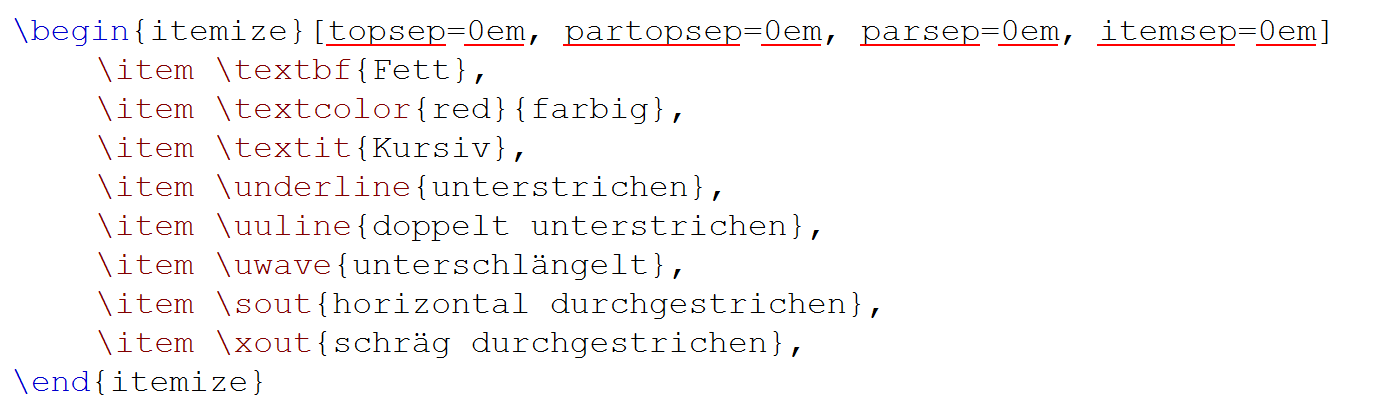
\includegraphics[width=0.75\textwidth]{./Bilder/TextBulletPointsStandard.png}}  
      \caption{Eigene Aufzählungszeichen}
\end{figure} 

Über die verschiedenen Seperatoren in der ersten Zeile, können die Abstände zwischen den einzelnen Aufzählungspunkten eingestellt werden. 


Die mit diesem Code erzeugte Aufzählung ist auf Seite \pageref{TextFormatieren} zu sehen.

\newpage Für Aufzählung mit selber definierten Aufzählungszeichen, ist folgende Code notwendig:

\begin{figure}[h!]
    \centering
      \fbox{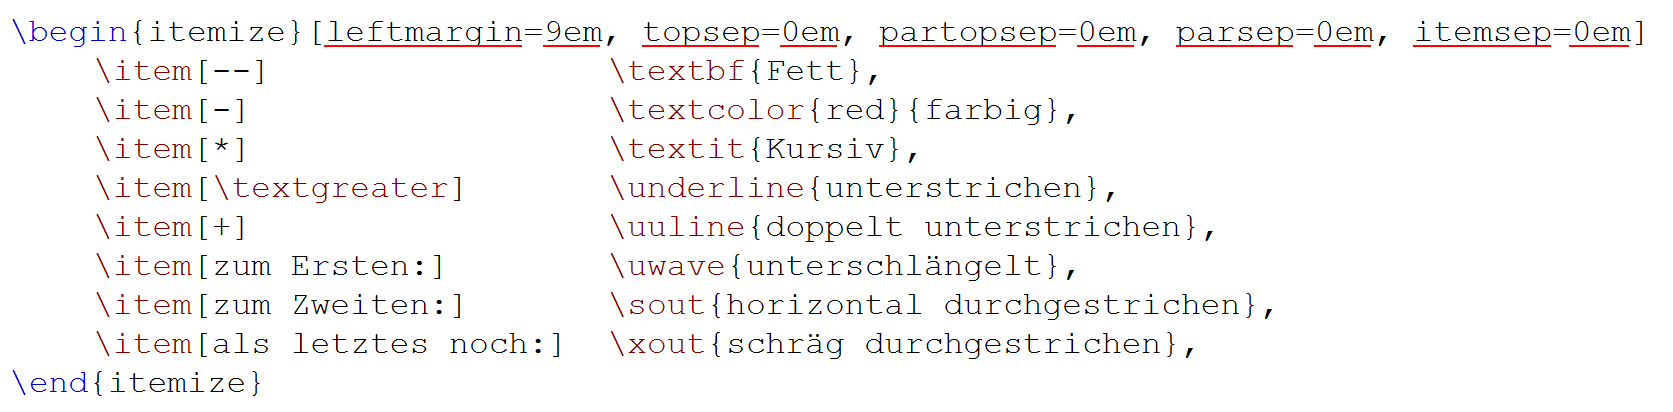
\includegraphics[width=0.75\textwidth]{./Bilder/TextBulletPoints.png}}  
      \caption{Eigene Aufzählungszeichen}
\end{figure} 

Auch hier werden über die verschiedenen Seperatoren in der ersten Zeile die Abstände zwischen den einzelnen Aufzählungspunkten eingestellt. Da in diesem Beispiel jedoch 'sehr lange' Aufzählungszeichen (z.B. 'als letztes noch') verwendet werden, muss die ganze Aufzählung deutlich mehr eingerückt werden (leftmargin=9em).  
 
Auch die mit diesem Code erzeugte Aufzählung ist auf Seite \pageref{TextFormatieren} zu sehen.

Dieses Beispiel zeigt, dass die Anzahl der Leerzeichen zwischen Worten resp, zwischen dem Aufzählungszeichen und den Worten keine Rolle spielt, da \LaTeX\ die Formatierung selber vornimmt.
